% Options for packages loaded elsewhere
\PassOptionsToPackage{unicode}{hyperref}
\PassOptionsToPackage{hyphens}{url}
%
\documentclass[
]{article}
\usepackage{amsmath,amssymb}
\usepackage{lmodern}
\usepackage{iftex}
\ifPDFTeX
  \usepackage[T1]{fontenc}
  \usepackage[utf8]{inputenc}
  \usepackage{textcomp} % provide euro and other symbols
\else % if luatex or xetex
  \usepackage{unicode-math}
  \defaultfontfeatures{Scale=MatchLowercase}
  \defaultfontfeatures[\rmfamily]{Ligatures=TeX,Scale=1}
\fi
% Use upquote if available, for straight quotes in verbatim environments
\IfFileExists{upquote.sty}{\usepackage{upquote}}{}
\IfFileExists{microtype.sty}{% use microtype if available
  \usepackage[]{microtype}
  \UseMicrotypeSet[protrusion]{basicmath} % disable protrusion for tt fonts
}{}
\makeatletter
\@ifundefined{KOMAClassName}{% if non-KOMA class
  \IfFileExists{parskip.sty}{%
    \usepackage{parskip}
  }{% else
    \setlength{\parindent}{0pt}
    \setlength{\parskip}{6pt plus 2pt minus 1pt}}
}{% if KOMA class
  \KOMAoptions{parskip=half}}
\makeatother
\usepackage{xcolor}
\usepackage[margin=1in]{geometry}
\usepackage{color}
\usepackage{fancyvrb}
\newcommand{\VerbBar}{|}
\newcommand{\VERB}{\Verb[commandchars=\\\{\}]}
\DefineVerbatimEnvironment{Highlighting}{Verbatim}{commandchars=\\\{\}}
% Add ',fontsize=\small' for more characters per line
\usepackage{framed}
\definecolor{shadecolor}{RGB}{248,248,248}
\newenvironment{Shaded}{\begin{snugshade}}{\end{snugshade}}
\newcommand{\AlertTok}[1]{\textcolor[rgb]{0.94,0.16,0.16}{#1}}
\newcommand{\AnnotationTok}[1]{\textcolor[rgb]{0.56,0.35,0.01}{\textbf{\textit{#1}}}}
\newcommand{\AttributeTok}[1]{\textcolor[rgb]{0.77,0.63,0.00}{#1}}
\newcommand{\BaseNTok}[1]{\textcolor[rgb]{0.00,0.00,0.81}{#1}}
\newcommand{\BuiltInTok}[1]{#1}
\newcommand{\CharTok}[1]{\textcolor[rgb]{0.31,0.60,0.02}{#1}}
\newcommand{\CommentTok}[1]{\textcolor[rgb]{0.56,0.35,0.01}{\textit{#1}}}
\newcommand{\CommentVarTok}[1]{\textcolor[rgb]{0.56,0.35,0.01}{\textbf{\textit{#1}}}}
\newcommand{\ConstantTok}[1]{\textcolor[rgb]{0.00,0.00,0.00}{#1}}
\newcommand{\ControlFlowTok}[1]{\textcolor[rgb]{0.13,0.29,0.53}{\textbf{#1}}}
\newcommand{\DataTypeTok}[1]{\textcolor[rgb]{0.13,0.29,0.53}{#1}}
\newcommand{\DecValTok}[1]{\textcolor[rgb]{0.00,0.00,0.81}{#1}}
\newcommand{\DocumentationTok}[1]{\textcolor[rgb]{0.56,0.35,0.01}{\textbf{\textit{#1}}}}
\newcommand{\ErrorTok}[1]{\textcolor[rgb]{0.64,0.00,0.00}{\textbf{#1}}}
\newcommand{\ExtensionTok}[1]{#1}
\newcommand{\FloatTok}[1]{\textcolor[rgb]{0.00,0.00,0.81}{#1}}
\newcommand{\FunctionTok}[1]{\textcolor[rgb]{0.00,0.00,0.00}{#1}}
\newcommand{\ImportTok}[1]{#1}
\newcommand{\InformationTok}[1]{\textcolor[rgb]{0.56,0.35,0.01}{\textbf{\textit{#1}}}}
\newcommand{\KeywordTok}[1]{\textcolor[rgb]{0.13,0.29,0.53}{\textbf{#1}}}
\newcommand{\NormalTok}[1]{#1}
\newcommand{\OperatorTok}[1]{\textcolor[rgb]{0.81,0.36,0.00}{\textbf{#1}}}
\newcommand{\OtherTok}[1]{\textcolor[rgb]{0.56,0.35,0.01}{#1}}
\newcommand{\PreprocessorTok}[1]{\textcolor[rgb]{0.56,0.35,0.01}{\textit{#1}}}
\newcommand{\RegionMarkerTok}[1]{#1}
\newcommand{\SpecialCharTok}[1]{\textcolor[rgb]{0.00,0.00,0.00}{#1}}
\newcommand{\SpecialStringTok}[1]{\textcolor[rgb]{0.31,0.60,0.02}{#1}}
\newcommand{\StringTok}[1]{\textcolor[rgb]{0.31,0.60,0.02}{#1}}
\newcommand{\VariableTok}[1]{\textcolor[rgb]{0.00,0.00,0.00}{#1}}
\newcommand{\VerbatimStringTok}[1]{\textcolor[rgb]{0.31,0.60,0.02}{#1}}
\newcommand{\WarningTok}[1]{\textcolor[rgb]{0.56,0.35,0.01}{\textbf{\textit{#1}}}}
\usepackage{graphicx}
\makeatletter
\def\maxwidth{\ifdim\Gin@nat@width>\linewidth\linewidth\else\Gin@nat@width\fi}
\def\maxheight{\ifdim\Gin@nat@height>\textheight\textheight\else\Gin@nat@height\fi}
\makeatother
% Scale images if necessary, so that they will not overflow the page
% margins by default, and it is still possible to overwrite the defaults
% using explicit options in \includegraphics[width, height, ...]{}
\setkeys{Gin}{width=\maxwidth,height=\maxheight,keepaspectratio}
% Set default figure placement to htbp
\makeatletter
\def\fps@figure{htbp}
\makeatother
\setlength{\emergencystretch}{3em} % prevent overfull lines
\providecommand{\tightlist}{%
  \setlength{\itemsep}{0pt}\setlength{\parskip}{0pt}}
\setcounter{secnumdepth}{-\maxdimen} % remove section numbering
\ifLuaTeX
  \usepackage{selnolig}  % disable illegal ligatures
\fi
\IfFileExists{bookmark.sty}{\usepackage{bookmark}}{\usepackage{hyperref}}
\IfFileExists{xurl.sty}{\usepackage{xurl}}{} % add URL line breaks if available
\urlstyle{same} % disable monospaced font for URLs
\hypersetup{
  pdftitle={Introduction to Tidyverse},
  pdfauthor={Jasmine Kobayashi},
  hidelinks,
  pdfcreator={LaTeX via pandoc}}

\title{Introduction to Tidyverse}
\author{Jasmine Kobayashi}
\date{09/07/2022}

\begin{document}
\maketitle

\hypertarget{introduction-to-the-tidyvrse-in-r}{%
\section{Introduction to the Tidyvrse in
R}\label{introduction-to-the-tidyvrse-in-r}}

Note that this notebook relies heavily on material from the textbook
\href{https://r4ds.had.co.nz/index.html}{R for Data Science} by Hadley
Wickham and Garrett Grolemund, and to a lesser extent, on the
\href{https://www.datacamp.com/courses/introduction-to-the-tidyverse}{DataCamp
course on the Tidyverse}. Both are great resources to explore!

\hypertarget{a.-what-is-the-tidyverse}{%
\subsection{A. What is the Tidyverse?}\label{a.-what-is-the-tidyverse}}

The Tidyverse is a collection of R packages meant to streamline data
science tasks. All Tidyverse packages share an underlying design
philosophy, grammar, and data structures. In this notebook, we'll learn
some basics of the Tidyverse. To install the tidyverse, open R Studio
and type install.packages(``tidyverse'', dependencies = TRUE). Then, for
each new session, you will need to load the Tidyverse:

\begin{Shaded}
\begin{Highlighting}[]
\CommentTok{\#install.packages("tidyverse", dependencies = TRUE)}
\FunctionTok{library}\NormalTok{(tidyverse)}
\end{Highlighting}
\end{Shaded}

\hypertarget{b.-some-very-basic-plotting-with-ggplot}{%
\subsection{B. Some (Very) Basic Plotting with
ggplot}\label{b.-some-very-basic-plotting-with-ggplot}}

Let's do some plotting with the mpg dataset. mpg contains observations
collected by the US Environmental Protection Agency on 38 models of
cars.

First, load and learn about the variables contained in this dataset. The
dataset is in the ggplot2 package, which is included in the tidyverse.
So, you can load the data using data(mpg).

\begin{Shaded}
\begin{Highlighting}[]
\FunctionTok{data}\NormalTok{(mpg)}
\FunctionTok{head}\NormalTok{(mpg)}
\end{Highlighting}
\end{Shaded}

\begin{verbatim}
## # A tibble: 6 x 11
##   manufacturer model displ  year   cyl trans      drv     cty   hwy fl    class 
##   <chr>        <chr> <dbl> <int> <int> <chr>      <chr> <int> <int> <chr> <chr> 
## 1 audi         a4      1.8  1999     4 auto(l5)   f        18    29 p     compa~
## 2 audi         a4      1.8  1999     4 manual(m5) f        21    29 p     compa~
## 3 audi         a4      2    2008     4 manual(m6) f        20    31 p     compa~
## 4 audi         a4      2    2008     4 auto(av)   f        21    30 p     compa~
## 5 audi         a4      2.8  1999     6 auto(l5)   f        16    26 p     compa~
## 6 audi         a4      2.8  1999     6 manual(m5) f        18    26 p     compa~
\end{verbatim}

Let's look at a plot that might tell us about the relationship between
drv (whether the car is front, rear, or 4-wheel drive) and hwy (highway
miles per gallon).

We begin a plot with the function ggplot(), which creates a coordinate
system that you can add layers to. Layers are created with ``+''
geom\_boxplot() will make a boxplot. In general, a template for creating
plots would be

\(\text{ggplot(data = DATA) + 
  <GEOM_FUNCTION>(mapping = aes(<MAPPINGS>))}\)

\textbf{Here's the basic code for the boxplot (fill in the correct
variables):}

\begin{Shaded}
\begin{Highlighting}[]
\CommentTok{\# changing this to a scatter plot }
\NormalTok{p\_scatter }\OtherTok{=} \FunctionTok{ggplot}\NormalTok{(}\AttributeTok{data =}\NormalTok{ mpg) }\SpecialCharTok{+} \FunctionTok{geom\_point}\NormalTok{(}\AttributeTok{mapping=}\FunctionTok{aes}\NormalTok{(}\AttributeTok{x=}\NormalTok{drv, }\AttributeTok{y=}\NormalTok{hwy))}
\CommentTok{\# using \textquotesingle{}equal{-}sign\textquotesingle{} because using function instead of value}
\NormalTok{p\_scatter}
\end{Highlighting}
\end{Shaded}

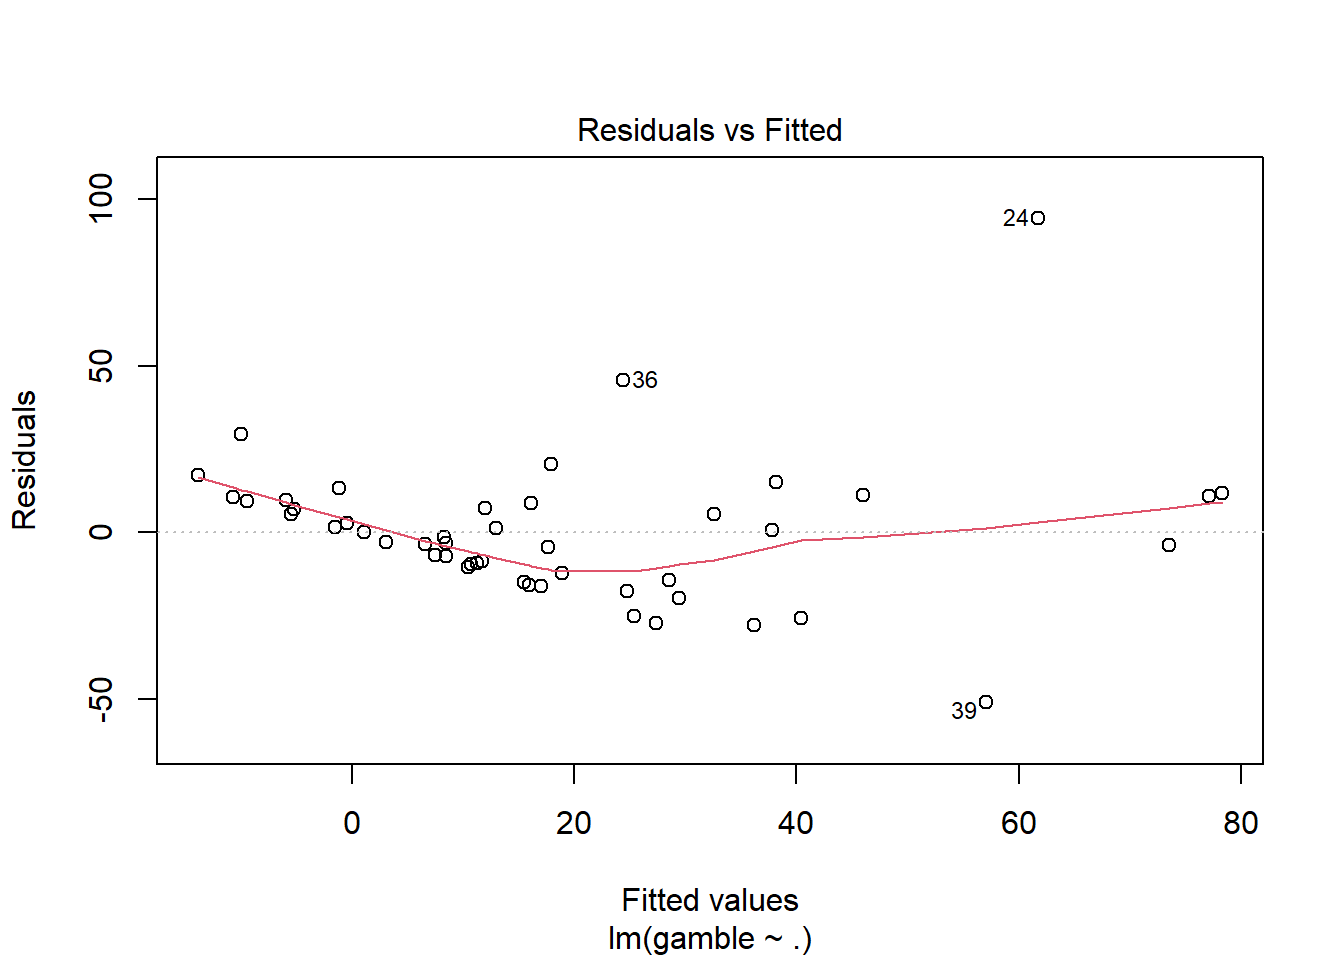
\includegraphics{Introduction-to-the-Tidyvrse-Class-Lecture_files/figure-latex/unnamed-chunk-3-1.pdf}

You can mess with \emph{all} sorts of things. For example, you could
change colors:

\begin{Shaded}
\begin{Highlighting}[]
\FunctionTok{ggplot}\NormalTok{(}\AttributeTok{data=}\NormalTok{mpg) }\SpecialCharTok{+} \FunctionTok{geom\_boxplot}\NormalTok{(}\AttributeTok{mapping =} \FunctionTok{aes}\NormalTok{(}\AttributeTok{x=}\NormalTok{drv, }\AttributeTok{y=}\NormalTok{hwy,}\AttributeTok{color=}\NormalTok{drv)) }\SpecialCharTok{+} \FunctionTok{scale\_color\_manual}\NormalTok{(}\AttributeTok{values=}\FunctionTok{c}\NormalTok{(}\StringTok{"\#999999"}\NormalTok{,}\StringTok{"\#E69F00"}\NormalTok{,}\StringTok{"\#56B4E9"}\NormalTok{))   }
\end{Highlighting}
\end{Shaded}

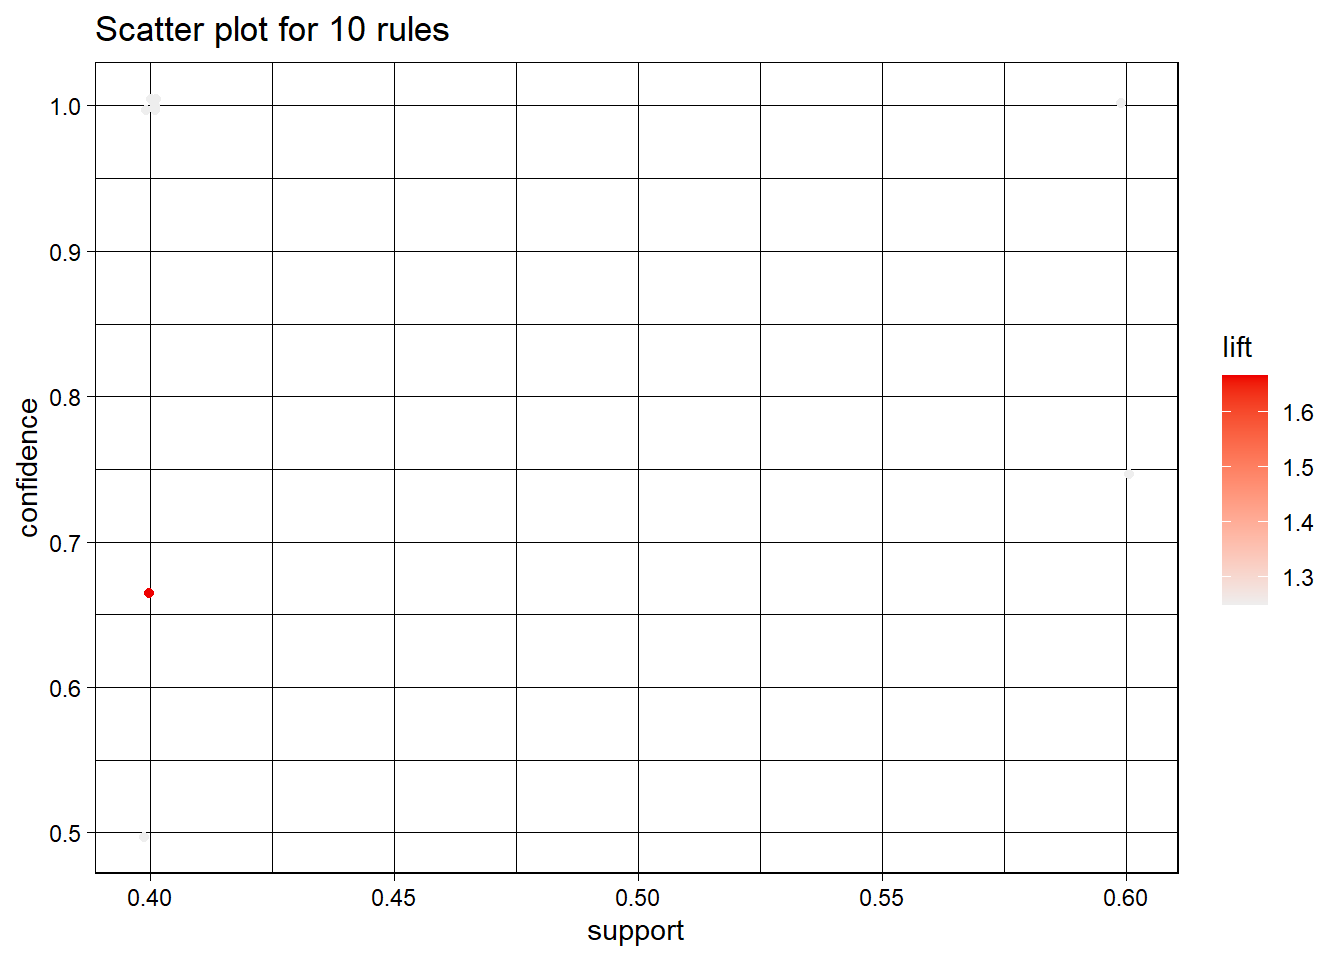
\includegraphics{Introduction-to-the-Tidyvrse-Class-Lecture_files/figure-latex/unnamed-chunk-4-1.pdf}

\begin{Shaded}
\begin{Highlighting}[]
\CommentTok{\# you can manually select specific color per category as above}
\end{Highlighting}
\end{Shaded}

\begin{Shaded}
\begin{Highlighting}[]
\FunctionTok{ggplot}\NormalTok{(}\AttributeTok{data=}\NormalTok{mpg) }\SpecialCharTok{+} 
  \FunctionTok{geom\_point}\NormalTok{(}\AttributeTok{mapping=} \FunctionTok{aes}\NormalTok{(}\AttributeTok{x =}\NormalTok{ displ, }\AttributeTok{y =}\NormalTok{ hwy, }\AttributeTok{color=}\NormalTok{drv))}
\end{Highlighting}
\end{Shaded}

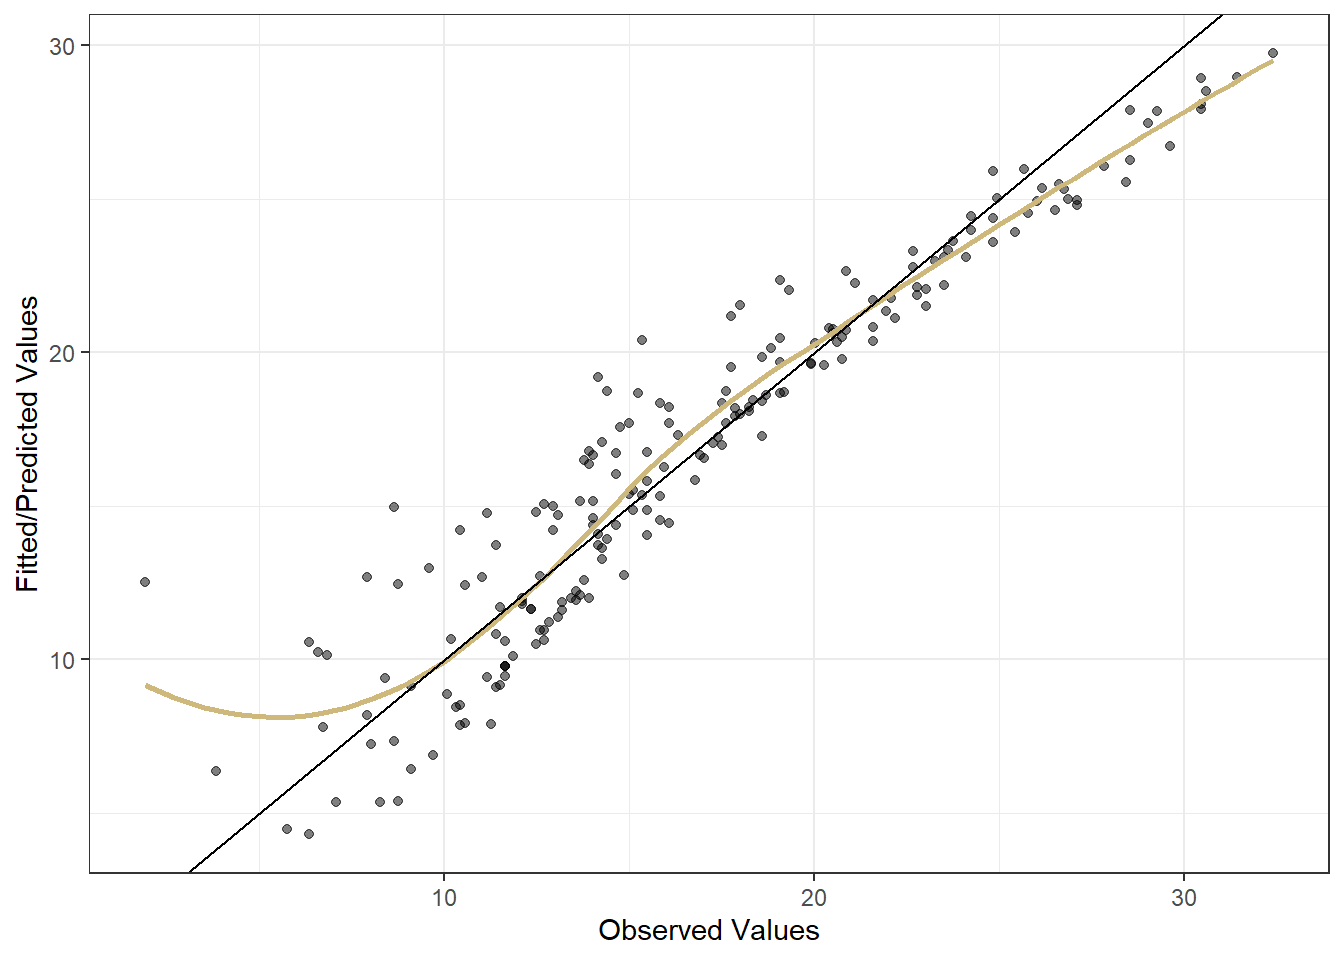
\includegraphics{Introduction-to-the-Tidyvrse-Class-Lecture_files/figure-latex/unnamed-chunk-5-1.pdf}

\textbf{What do we notice about the relationship between engine
displacement and hwy miles per gallon?}

There is a downward trending \texttt{hwy} as \texttt{displ} increases.
This trend appears roughly, linear. However, there may be some evidence
of curvature at the extremes of the \texttt{displ}

\textbf{What do we notice?}

\begin{itemize}
\item
  The relationship between \texttt{hwy} and \texttt{displ} is grouped by
  \texttt{drv}.
\item
  We also notice a downward trend between\texttt{hwy} and \texttt{displ}
  in each group (thought it seems like a weak downward trend for rear
  wheel drive).
\item
  On average, front wheel drive cars with low engine displacement have
  the highest highyway mpg. On the contrary, rear wheel drive cars with
  high engine displacement have the lowest highway mpg.
\end{itemize}

Another way to add information from a categorical variable to plots is
by using \emph{facets}. Facets split a plot into subplots, such that
each subplot contains data for a particular level of the categorical
variable.

We can facet by adding the function
\texttt{facet\_wrap(\textasciitilde{}\ Catvar,\ nrow=x} to our ggplot.
Where, \texttt{Catvar} is the categorical variable that we want to facet
on , and \texttt{x} is the number of rows that we'd like (we could also
\texttt{ncol}\ldots)

\emph{Create a facet plot where you split the data based on the class
variable}

\begin{Shaded}
\begin{Highlighting}[]
\NormalTok{p\_facet }\OtherTok{=} \FunctionTok{ggplot}\NormalTok{(}\AttributeTok{data=}\NormalTok{mpg) }\SpecialCharTok{+} 
  \FunctionTok{geom\_point}\NormalTok{(}\AttributeTok{mapping =} \FunctionTok{aes}\NormalTok{(}\AttributeTok{x=}\NormalTok{displ, }\AttributeTok{y=}\NormalTok{hwy)) }\SpecialCharTok{+}
  \FunctionTok{facet\_wrap}\NormalTok{( }\SpecialCharTok{\textasciitilde{}}\NormalTok{ class, }\AttributeTok{nrow=}\DecValTok{2}\NormalTok{)}
\NormalTok{p\_facet}
\end{Highlighting}
\end{Shaded}

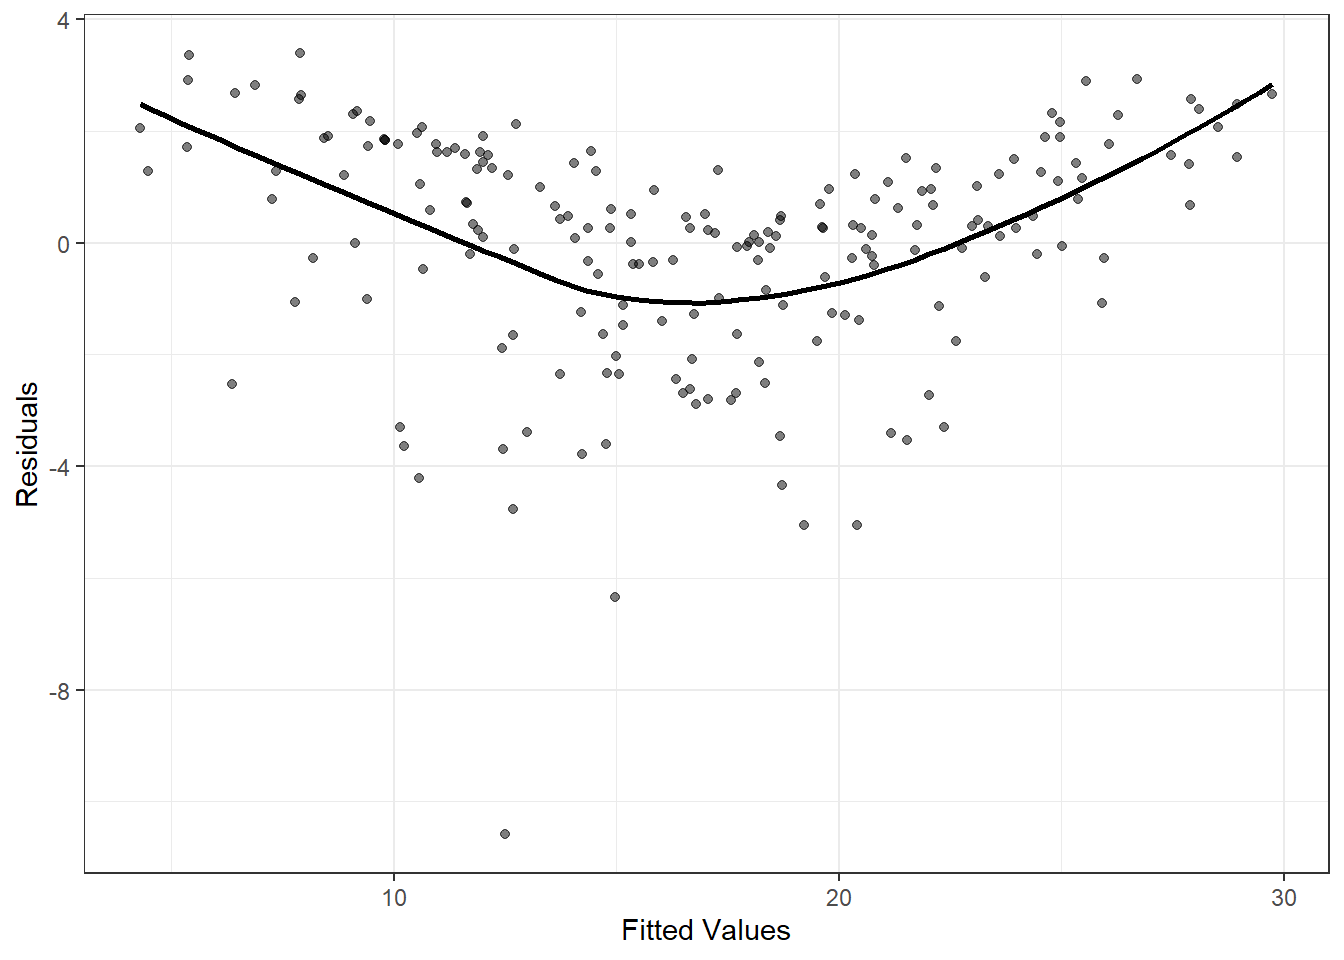
\includegraphics{Introduction-to-the-Tidyvrse-Class-Lecture_files/figure-latex/unnamed-chunk-6-1.pdf}

Instead of seeing the individual data points, we might be interested in
visualizing some overall trend between displ and hwy. We could do this
by substituting geom\_points() with geom\_smooth(). \textbf{Try it!}

\begin{Shaded}
\begin{Highlighting}[]
\FunctionTok{ggplot}\NormalTok{(}\AttributeTok{data=}\NormalTok{mpg) }\SpecialCharTok{+} \FunctionTok{geom\_smooth}\NormalTok{(}\AttributeTok{mapping =} \FunctionTok{aes}\NormalTok{(}\AttributeTok{x=}\NormalTok{displ, }\AttributeTok{y=}\NormalTok{hwy, }\AttributeTok{color=}\StringTok{\textquotesingle{}red\textquotesingle{}}\NormalTok{))}
\end{Highlighting}
\end{Shaded}

\begin{verbatim}
## `geom_smooth()` using method = 'loess' and formula 'y ~ x'
\end{verbatim}

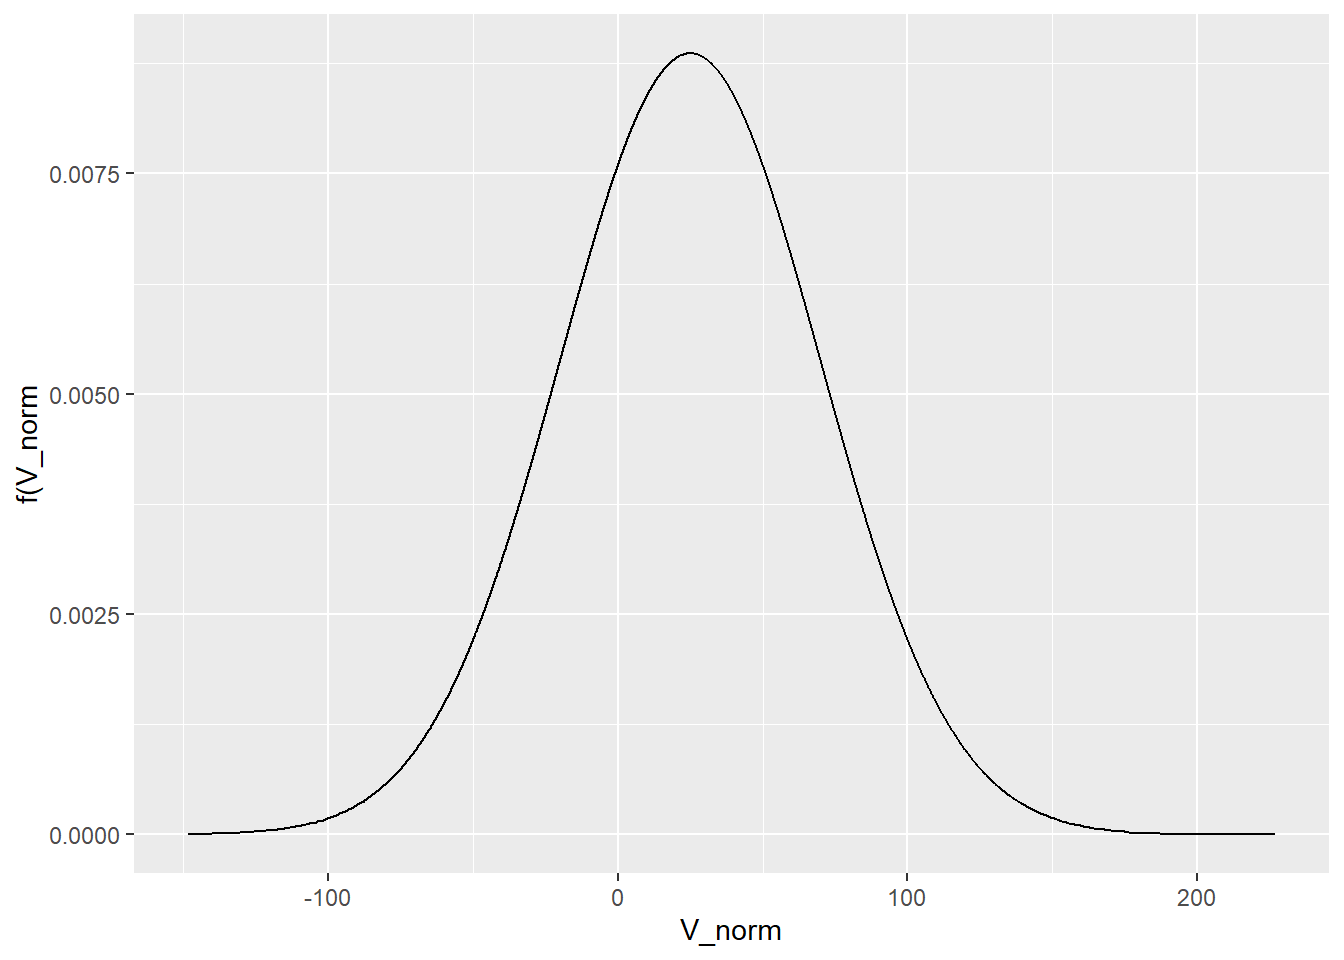
\includegraphics{Introduction-to-the-Tidyvrse-Class-Lecture_files/figure-latex/unnamed-chunk-7-1.pdf}

And, we can layer the smooth over the scatterplot pretty easily by
adding ``+ geom\_point()''. \textbf{Try it!}

\begin{Shaded}
\begin{Highlighting}[]
\FunctionTok{ggplot}\NormalTok{(}\AttributeTok{data=}\NormalTok{mpg) }\SpecialCharTok{+} \FunctionTok{geom\_smooth}\NormalTok{(}\AttributeTok{mapping =} \FunctionTok{aes}\NormalTok{(}\AttributeTok{x=}\NormalTok{displ, }\AttributeTok{y=}\NormalTok{hwy, }\AttributeTok{color=}\StringTok{\textquotesingle{}red\textquotesingle{}}\NormalTok{)) }\SpecialCharTok{+} \FunctionTok{geom\_point}\NormalTok{(}\AttributeTok{mapping =} \FunctionTok{aes}\NormalTok{(}\AttributeTok{x=}\NormalTok{displ, }\AttributeTok{y=}\NormalTok{hwy,))}
\end{Highlighting}
\end{Shaded}

\begin{verbatim}
## `geom_smooth()` using method = 'loess' and formula 'y ~ x'
\end{verbatim}

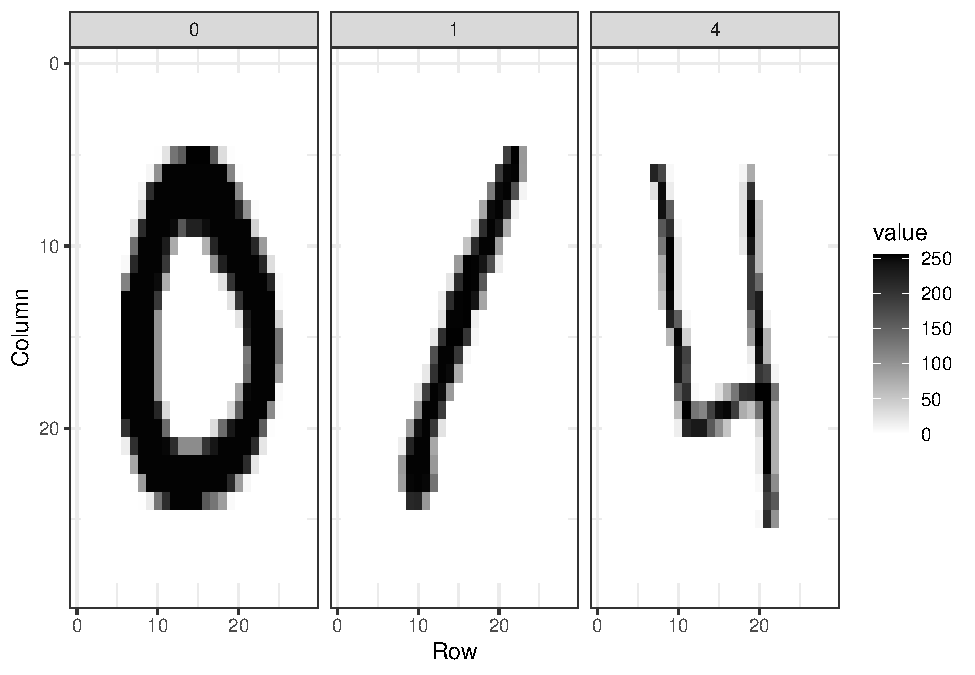
\includegraphics{Introduction-to-the-Tidyvrse-Class-Lecture_files/figure-latex/unnamed-chunk-8-1.pdf}

\hypertarget{c.-data-manipulation-and-transformation}{%
\subsection{C. Data Manipulation and
Transformation}\label{c.-data-manipulation-and-transformation}}

\texttt{dplyr} is a package in the Tidyverse that provides simple
``verbs'', or functions that correspond to the most common data
manipulation tasks, to help you translate your thoughts into code. Let's
see how some of these verbs work on the gapminder dataset.
\textbf{First, if you haven't already, let's install and load the
gapminder package.}

\begin{Shaded}
\begin{Highlighting}[]
\CommentTok{\#install.packages("gapminder")}
\FunctionTok{library}\NormalTok{(gapminder)}
\FunctionTok{library}\NormalTok{(dplyr)}
\end{Highlighting}
\end{Shaded}

\textbf{Write a summary of the variables in this dataset. }

\begin{Shaded}
\begin{Highlighting}[]
\FunctionTok{data}\NormalTok{(gapminder)}
\FunctionTok{head}\NormalTok{(gapminder)}
\end{Highlighting}
\end{Shaded}

\begin{verbatim}
## # A tibble: 6 x 6
##   country     continent  year lifeExp      pop gdpPercap
##   <fct>       <fct>     <int>   <dbl>    <int>     <dbl>
## 1 Afghanistan Asia       1952    28.8  8425333      779.
## 2 Afghanistan Asia       1957    30.3  9240934      821.
## 3 Afghanistan Asia       1962    32.0 10267083      853.
## 4 Afghanistan Asia       1967    34.0 11537966      836.
## 5 Afghanistan Asia       1972    36.1 13079460      740.
## 6 Afghanistan Asia       1977    38.4 14880372      786.
\end{verbatim}

\hypertarget{filter-rows-with-filter}{%
\subsubsection{Filter rows with
filter()}\label{filter-rows-with-filter}}

It is often useful to study a subset of your data.

The verb \texttt{filter()} will easily allow you to filter rows
(observations) in a data frame. Here's one possibility:

Piping Function: \texttt{\%\textgreater{}}

\begin{Shaded}
\begin{Highlighting}[]
\CommentTok{\#filter(gapminder, country == "United States")}
\CommentTok{\#or}

\NormalTok{gapminder }\SpecialCharTok{\%\textgreater{}\%}
  \FunctionTok{filter}\NormalTok{(country }\SpecialCharTok{==} \StringTok{"United States"}\NormalTok{)}
\end{Highlighting}
\end{Shaded}

\begin{verbatim}
## # A tibble: 12 x 6
##    country       continent  year lifeExp       pop gdpPercap
##    <fct>         <fct>     <int>   <dbl>     <int>     <dbl>
##  1 United States Americas   1952    68.4 157553000    13990.
##  2 United States Americas   1957    69.5 171984000    14847.
##  3 United States Americas   1962    70.2 186538000    16173.
##  4 United States Americas   1967    70.8 198712000    19530.
##  5 United States Americas   1972    71.3 209896000    21806.
##  6 United States Americas   1977    73.4 220239000    24073.
##  7 United States Americas   1982    74.6 232187835    25010.
##  8 United States Americas   1987    75.0 242803533    29884.
##  9 United States Americas   1992    76.1 256894189    32004.
## 10 United States Americas   1997    76.8 272911760    35767.
## 11 United States Americas   2002    77.3 287675526    39097.
## 12 United States Americas   2007    78.2 301139947    42952.
\end{verbatim}

**Filter

\hypertarget{arranging-with-arrange}{%
\subsubsection{Arranging with arrange()}\label{arranging-with-arrange}}

\textbf{Use the arrange() verb, in conjunction with the code above to
put the United States data in descending order with respect to year.}

\begin{Shaded}
\begin{Highlighting}[]
\NormalTok{gapminder }\SpecialCharTok{\%\textgreater{}\%} \FunctionTok{filter}\NormalTok{(country }\SpecialCharTok{==} \StringTok{"United States"}\NormalTok{) }\SpecialCharTok{\%\textgreater{}\%} \FunctionTok{arrange}\NormalTok{(}\FunctionTok{desc}\NormalTok{(year))}
\end{Highlighting}
\end{Shaded}

\begin{verbatim}
## # A tibble: 12 x 6
##    country       continent  year lifeExp       pop gdpPercap
##    <fct>         <fct>     <int>   <dbl>     <int>     <dbl>
##  1 United States Americas   2007    78.2 301139947    42952.
##  2 United States Americas   2002    77.3 287675526    39097.
##  3 United States Americas   1997    76.8 272911760    35767.
##  4 United States Americas   1992    76.1 256894189    32004.
##  5 United States Americas   1987    75.0 242803533    29884.
##  6 United States Americas   1982    74.6 232187835    25010.
##  7 United States Americas   1977    73.4 220239000    24073.
##  8 United States Americas   1972    71.3 209896000    21806.
##  9 United States Americas   1967    70.8 198712000    19530.
## 10 United States Americas   1962    70.2 186538000    16173.
## 11 United States Americas   1957    69.5 171984000    14847.
## 12 United States Americas   1952    68.4 157553000    13990.
\end{verbatim}

\hypertarget{selecting-columns-with-select}{%
\subsubsection{Selecting columns with
select()}\label{selecting-columns-with-select}}

In addition to being able to filter out a subset of rows, you can also
filter out a subset of columns with the select() verb. \textbf{Try to
select just the country and year variables.}

\begin{Shaded}
\begin{Highlighting}[]
\FunctionTok{head}\NormalTok{(}\FunctionTok{select}\NormalTok{(gapminder,country,year))}
\end{Highlighting}
\end{Shaded}

\begin{verbatim}
## # A tibble: 6 x 2
##   country      year
##   <fct>       <int>
## 1 Afghanistan  1952
## 2 Afghanistan  1957
## 3 Afghanistan  1962
## 4 Afghanistan  1967
## 5 Afghanistan  1972
## 6 Afghanistan  1977
\end{verbatim}

\hypertarget{changing-columns-with-mutate}{%
\subsubsection{Changing columns with
mutate()}\label{changing-columns-with-mutate}}

We can also mutate certain columns. For example, suppose that we wanted
life expectancy to be measured in months. We might write:

\begin{Shaded}
\begin{Highlighting}[]
\FunctionTok{head}\NormalTok{(gapminder }\SpecialCharTok{\%\textgreater{}\%} \FunctionTok{mutate}\NormalTok{(}\AttributeTok{life\_expectancy =}\NormalTok{ life\_expectancy}\SpecialCharTok{*}\DecValTok{12}\NormalTok{))}
\end{Highlighting}
\end{Shaded}

\textbf{Create a new column in the data frame that is just GDP (not GDP
per capita).}

\begin{Shaded}
\begin{Highlighting}[]
\NormalTok{gapminder\_GDP }\OtherTok{=} \FunctionTok{head}\NormalTok{(gapminder }\SpecialCharTok{\%\textgreater{}\%} \FunctionTok{mutate}\NormalTok{(}\AttributeTok{gdp =}\NormalTok{ gdpPercap}\SpecialCharTok{*}\NormalTok{pop)) }\CommentTok{\#has a new column \textquotesingle{}gdp\textquotesingle{}}
\NormalTok{gapminder\_GDP                                                   }\CommentTok{\#name of new a df}
\end{Highlighting}
\end{Shaded}


\end{document}
